\documentclass[a4paper,11pt]{jlreq}
% 基本とドライバ関連
\usepackage{graphicx}
\usepackage{xcolor}
\usepackage{makeidx}
\usepackage{ascmac}

% LuaTeX-ja設定
\usepackage{luatexja}% 日本語したい
\usepackage[haranoaji,no-math,deluxe,expert,nfssonly,match,scale=1.0]{luatexja-preset}
\renewcommand{\kanjifamilydefault}{\gtdefault}% 既定をゴシック体に
\usepackage{lltjext}

% 数式系基本
\usepackage{amsmath}
\usepackage{amsthm}
\usepackage{amssymb}
\usepackage{mathtools}
% \mathtoolsset{showonlyrefs=true}
\usepackage{derivative}
\usepackage[b]{esvect}
\usepackage{nicematrix}
\usepackage{siunitx}
\usepackage{bm}

% 画像関係
\usepackage{animate}
\usepackage{svg}
\usepackage{tikz}

%表関連
\usepackage{multirow}

% 自然科学用追加
% \usepackage{chemmacros}
% \usechemmodule{all}
% \selectchemgreekmapping{fontspec}
\usepackage{chemfig}
\setchemfig{atom sep=1.5em}
% \ifdraft{}{\setchemfig{bond join=true}}

% 数式フォント設定
\usepackage{anyfontsize}
\newcommand{\sfscale}{0.98}
\newcommand{\ttscale}{0.96}
% \usepackage[mathnoalias]{iwona}
% % \setmainfont{Iwona}
% \usepackage[scale=\sfscale]{roboto}
% \usepackage[scale=\ttscale]{roboto-mono}
% \usepackage{BOONDOX-uprscr}
% \usepackage{BOONDOX-ds}

% ページ設定
\usepackage{geometry}
\geometry{left=25truemm, right=25truemm, top=25truemm, bottom=25truemm}
% \pagestyle{empty}

% hyperref関連
\usepackage{bookmark}
\usepackage{xurl}
\hypersetup{unicode,bookmarksnumbered=true,colorlinks=true,final}

%%%%%%%%%%%%%%%%%%%%%%%
\graphicspath{{../figure/}{../../figure/}}

\begin{document}
\section{高分子鎖のモデルと実在鎖との関係}

\ref{sec:CG_model} 章で、実在の高分子鎖を大幅に簡略化した「自由連結鎖」、あるいは、ある程度結合状態を考慮した「自由回転鎖」および「束縛回転鎖」モデルを用いた末端間距離 $R$ および慣性半径 $R_g$ についての議論を行った。
ここでは、実際の測定により得られる慣性半径および分子量と上記モデルからの理論値とを繋げていく議論を進めよう。


\subsection{特性比について}

任意のセグメント数 $n$ である場合の末端間距離の実測値と自由連結鎖モデルでの理論値とを、以下のように比較することを考えよう。
\begin{align}
C_n=\dfrac{ \langle R_n^2 \rangle }{n b^2}
\end{align}
なお、理想鎖として取り扱えるように$\theta$状態で末端間距離を実測し、ボンド長さ $b$ は C-C 結合の 1.54 \AA を用いる。

この値は、自由連結鎖と比較して実在鎖がどのぐらい膨らんでいるかを表しており、一般にセグメント数の増加に伴い増加し、やがて、一定値に収束することが確かめられている。
したがって、特性比 $C_{\infty}$ は、上記の値を分子量を無限大に外挿した形で、以下のように定義されている。
\begin{align}
C_{\infty}=\lim_{n \to \infty} C_n 
%= \dfrac{ \langle R_N^2 \rangle }{N b^2}=\lim_{N \to \infty} \dfrac{ 6 \langle R_g^2 \rangle }{N b^2}
\label{eq:Cinf}
\end{align}
しかしながら、実際に分子量を無限大にするわけではなく、ある程度以上大きな繰り返し数のポリマーの慣性半径を数点実測することにより一定に収束していることを確認すればよい。

これまでの議論では、仮想的なモデルとしてセグメントの数 $N$ を設定して議論を行ってきた。
ここに、実測の分子量から見積もった重合度 $DP$(Degree of Polymerization: ポリマーの分子量をモノマーの分子量で除した値であり、モノマーの繰り返し数)を使用することで、仮想的なモデルと実在鎖との相関を議論することができる。
なお、この時の分子量としては重量平均分子量 $M_w$ を用いることが妥当である。

\begin{align}
C_{\infty} = \lim_{DP \to \infty} \dfrac{ \text{二乗平均末端間距離の実測値} }{DP \times b^2}
\label{fig:CR}
\end{align}

慣性半径 $R_g$ は実測可能であるので、これを用いて上式中の二乗平均末端間距離の実測値を求めると、例えばポリエチレンで $C_{\infty} \simeq 6.7$ 程度の値となっている。
すなわち、自由連結モデルよりも実在鎖は 7 倍程度膨らんでいるわけであり、この原因はボンドの角度に束縛が入っているためと考えることができる。

例えば、束縛回転鎖モデルでは、(\ref{eq:r2_sokubaku}) 式の $\dfrac{1+\cos \theta}{1-\cos \theta} \dfrac{1+ \langle \cos \theta \rangle}{1- \langle \cos \theta \rangle}$ の因子が、$C_{\infty}$ に対応することになり、トランスとゴーシュの排除が入ることを考慮するとこの値は 4 程度と計算され、1,5 位の相互作用であるペンタン効果を考慮することで、ほぼ実測と近い結果が得られるようである。

また、この特性比は、高分子鎖に置換基が入ることで増加し、かさ高いフェニル基を有するポリスチレンでは、10 程度となっている。



\subsection{有効結合長}

ここまでの自由連結鎖の議論において用いてきたボンド(ボンド長さ $b$)を m 個まとめて、新たなボンドとしてボンド長が $a$ となるボンドベクトルを考えよう。
%このとき、
%\begin{align}
%{\bf a}_i = 
%\end{align}
図 \ref{fig: EBL} にそのイメージを示した。
黒矢印で描かれた元のボンド(ボンド長さ $b$)に対して、青色で示した新たなボンド(ボンド長が $a$)を末端間ベクトル(図中の赤矢印)が同一となるように定義することができる。
\begin{figure}[htb]
 \centering
	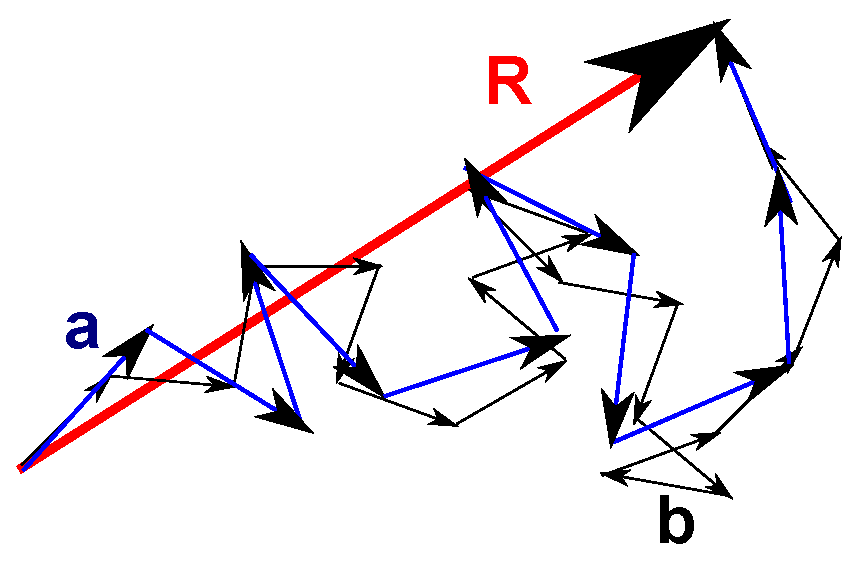
\includegraphics[width=6cm]{EBL.eps}
	\caption{有効結合長 a のイメージ}
	\label{fig: EBL}
\end{figure}

ここでは、末端間ボンドベクトル\bm{R}が変化しないように同一の高分子鎖上に新たなボンドベクトル\bm{a}を設定しているのであるから、新たなセグメント数 $N'=\dfrac{N}{m}$ を用いて、以下となる。
\begin{align}
&\langle R^2 \rangle = N b^2 = N' a^2 = \left(\dfrac{N}{m}\right) a^2 \notag \\
\therefore \quad &a = m^{1/2} b
\label{eq:EBL}
\end{align}

m は 1 以上の任意の数を設定することができ、このように設定した $a$ のことを有効結合長と呼ぶ。 
m の取り方によって、高分子鎖のそれぞれのボンド長さの総和、すなわち、$Nb$ で表される伸び切った鎖の長さは変化することになる。
これは、鎖に沿ったように見た場合の粗視化の度合いを表していることになり、m=N の極限では、伸び切り鎖長は末端間距離と等しいことになる。

図 \ref{fig: RF} に示した 1000 セグメントからなる自由連結鎖を、100 セグメントごとにまとめて 10 セグメントに粗視化し、元の 100 セグメントの重心を中心に有効結合長を直径とする円で表したものを図 \ref{fig: RF_CG} に示した。
\begin{figure}[htb]
 \centering
	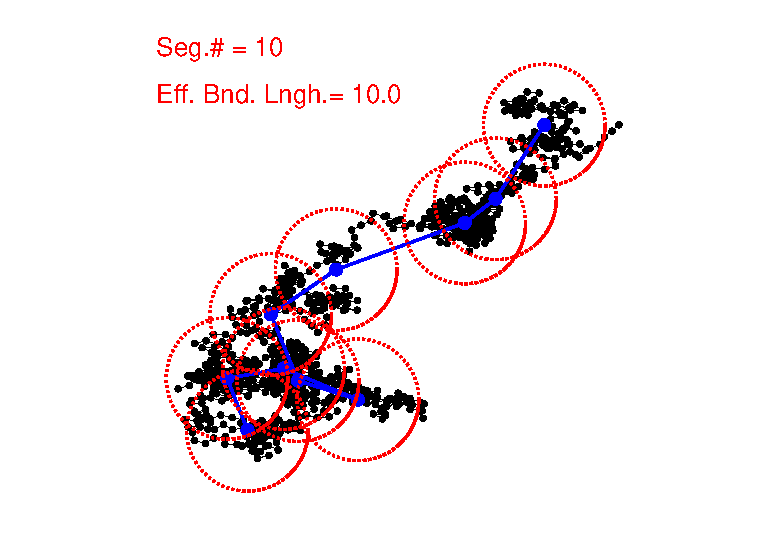
\includegraphics[width=10cm]{RF_CG.eps}
	\caption{粗視化セグメントのイメージ}
	\label{fig: RF_CG}
\end{figure}

これまでの議論では暗黙の裡に、新たなボンドベクトルが同一のボンド長を有するように記述してきたが、この設定は以下に示したような二種類のやり方を考えることができる
\begin{enumerate}
\item
結節点の位置を再現するように、それぞれのボンド長が異なる新たなボンドベクトル ${\bm a}_k$ を設定。
\begin{align*}
{\bm a}_k = \sum_{i=kN/m}^{kN/m + m-1} {\bm b}_i 
\end{align*}
\item
(\ref{eq:EBL}) 式で定義したボンド長$a$となる新たなボンドベクトルを末端間ボンドベクトル\bm{R}が変化しないように同一の高分子鎖上に設定する。
このとき、結節点の位置は再現できないことになる。
\end{enumerate}

このようなスケールのとり直しを、実測値により得られた (\ref{fig:CR}) 式の特性比を用いて行うと、
\begin{align}
\text{二乗平均末端間距離の実測値} &= C_{\infty} \times DP \times b^2 = DP \times a^2 \notag \\
\therefore \quad a &= C_{\infty}^{1/2} b
\end{align}
となり、実在の高分子鎖を有効結合長 a の自由連結鎖として表すことができるようになる。

\subsection{クーン長}

有効結合長という考え方を使った定義として、Kuhn が提案したクーン長($b_k$)がある。

これは、前節と同様に実在鎖に対して有効結合長を定義する際に、以下のように伸び切り鎖の長さが同一となるという境界条件を付与して、$N_k$ 個のセグメントに取り直すという定義である。
この定義の意味は、高分子鎖に沿ってみた場合の長さを変化させないという意味で、粗視化する際の最小限の単位長さを表していると考えることができる。
\begin{align}
 \begin{cases}
	C_{\infty} DP \times b^2 = N_k b_k^2 \\
	DP \times b = N_k b_k
 \end{cases}
\end{align}

具体的な値としては、この連立方程式を解いて、
\begin{align}
b_k = C_{\infty} b \notag \\
N_k = \dfrac{N}{C_{\infty} }
\end{align}
となる。

\end{document}